\section{Results and analysis}
\subsection{E1: the integer boundary determines broadcast recovery}
Figure~\ref{fig:e1} shows all 28 sample--subset combinations across the 20 key-set blocks. Every one of the 560 rows agreed with the prediction $M^3<N_S$. The minimum number of intercepted ciphertexts was one for \texttt{B}$\times1$, two for \texttt{B}$\times96$, three for \texttt{B}$\times180$, and one for the leading-zero 96-byte sample. For these keys, all three two-recipient choices recover the \texttt{B}$\times96$ integer, whereas only the full three-recipient set recovers \texttt{B}$\times180$. Selection matters through the product $N_S$, rather than through a fixed positional rule. The very short message can be recovered from one ciphertext because its cube already lies below one 2048-bit modulus.

\begin{figure}[!ht]
\centering
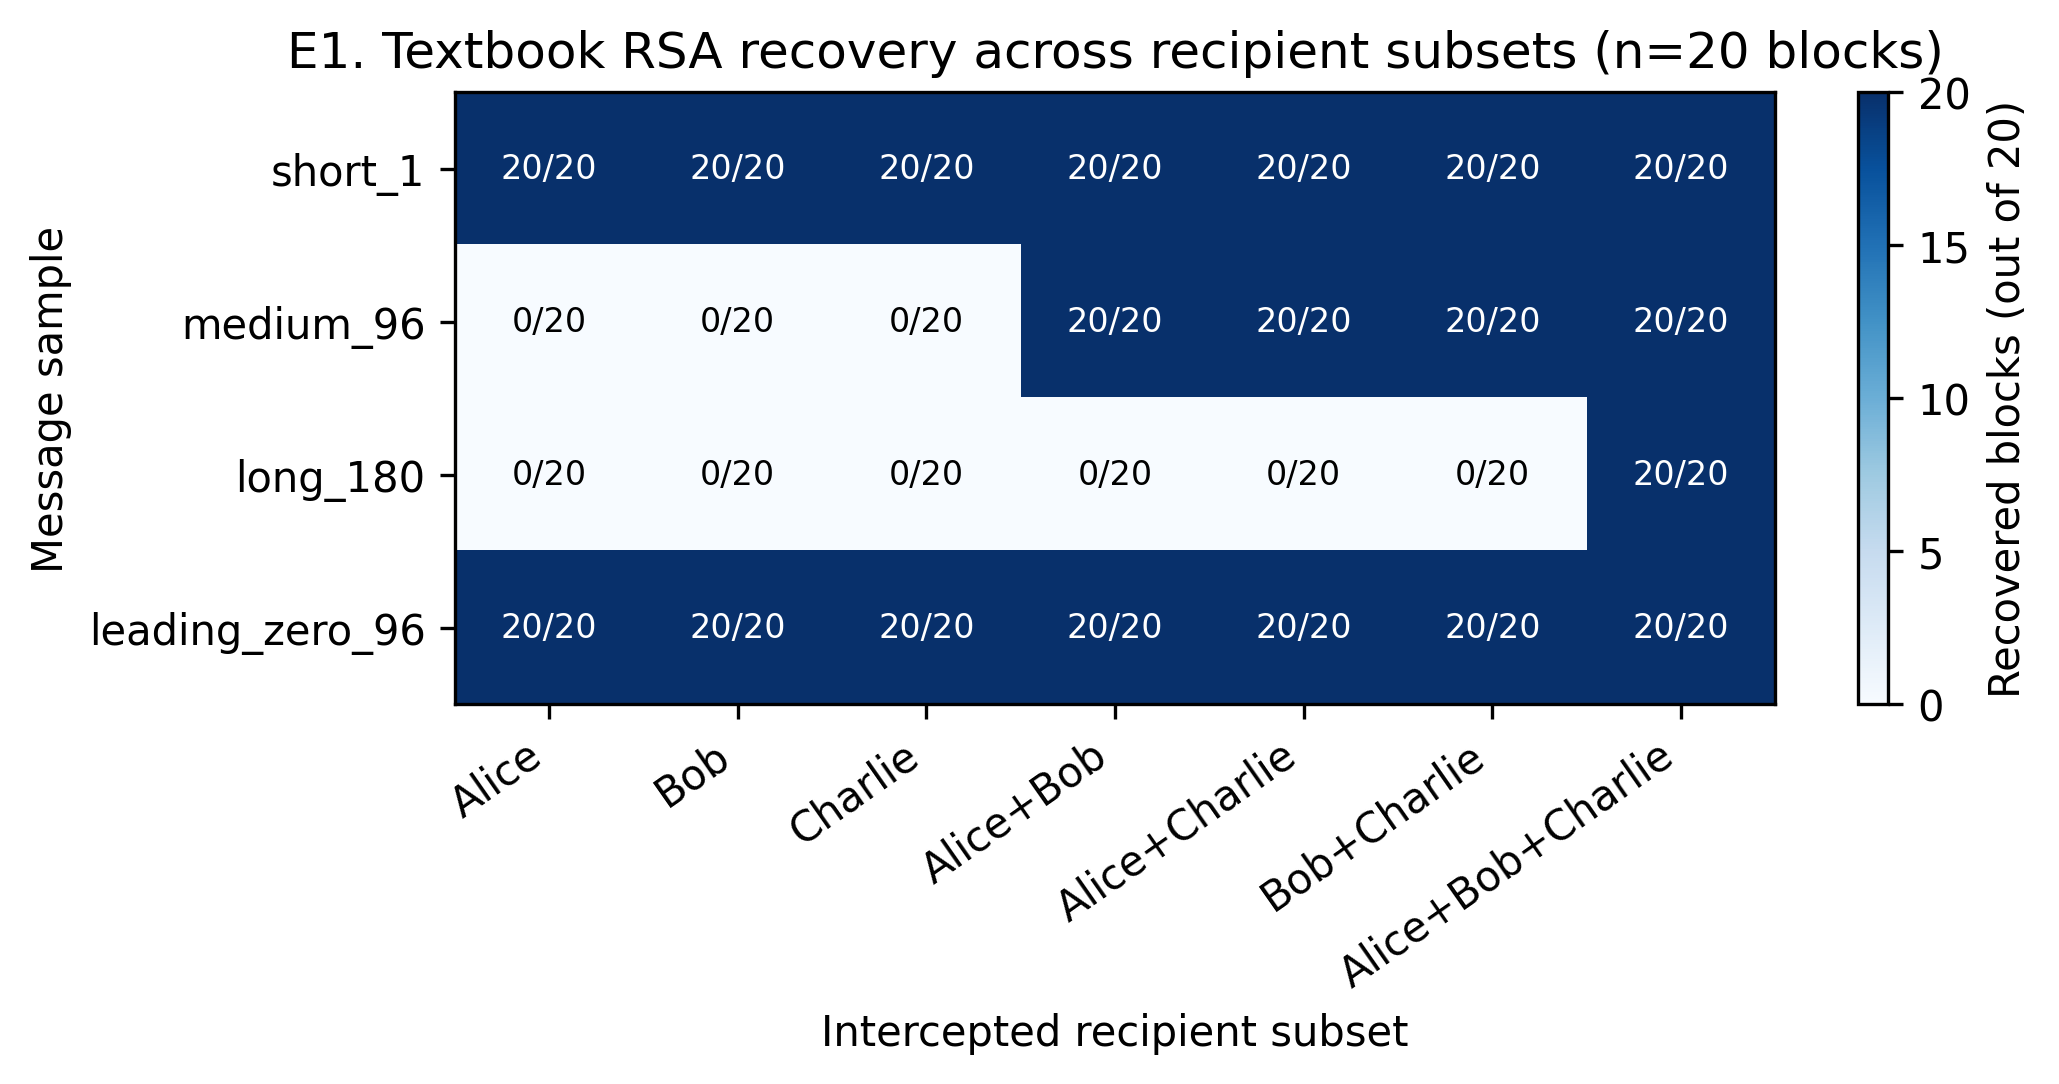
\includegraphics[width=\linewidth]{../docs/analysis/figures/figure_1_e1_recovery_matrix.png}
\caption{Evaluator-confirmed \emph{integer} recovery for four fixed textbook RSA messages and all seven nonempty recipient subsets; each cell is successful key-set blocks out of 20. The two 96-byte rows encode different integers. The leading-zero row's original 96-byte serialization is not inferred by Eve without independent length information.}
\label{fig:e1}
\end{figure}

Although both samples occupy 96 bytes, \texttt{B}$\times96$ is a 767-bit integer and $\texttt{0x00}^{95}\Vert\texttt{0x02}$ equals 2. Eve can recover 2 from one ciphertext but cannot infer its original byte length; the plotted success metric is evaluator-confirmed integer equality.
\FloatBarrier

\subsection{E2: paired textbook RSA and OAEP comparison}
Table~\ref{tab:e2} summarizes the 60 paired tests. Each pair holds plaintext, three RSA keypairs, $e=3$, recipient set and CRT-and-root attacker fixed. Textbook RSA presented the repeated integer relation, and the tested procedure returned the original integer in every pair. OAEP randomized the encoded representatives before RSA exponentiation; the same procedure recovered the original plaintext in no paired test. Legitimate OAEP decryption succeeded in every pair, and repeated OAEP encryptions under the same key yielded distinct ciphertexts in all 60 checks.

\begin{table}[!ht]
\centering
\caption{E2 paired observations across 20 independent RSA key-set blocks and three messages per block. ``Attack recovery'' means evaluator-confirmed equality with the original message; legitimate decryption is a different operation.}
\label{tab:e2}
\begin{tabular}{@{}lll@{}}
\toprule
Scheme & Evaluated operation & Correct / 60 pairs \\
\midrule
Textbook RSA & Eve's CRT-and-root recovery & 60/60 \\
RSA-OAEP & Eve's same CRT-and-root recovery & 0/60 \\
RSA-OAEP & Intended recipients' decryption & 60/60 \\
\bottomrule
\end{tabular}
\end{table}

Using the same keys prevents a changing modulus set from explaining the within-pair contrast. The observations do not prove RSA-OAEP secure against every attack, nor do 60 comparisons represent 60 independent key sets. They establish a narrower result: the controlled CRT-and-root procedure that exploits a shared unpadded $M$ did not recover the OAEP plaintext in these trials. OAEP's randomized encoding is specified by RFC~8017~\cite{moriarty2016pkcs1}; repeated-ciphertext diversity is illustrative evidence of that behavior, not a security reduction.
\FloatBarrier

\subsection{E3: cryptographic work, serialization and package size}
Figure~\ref{fig:e3} separates \emph{encrypt+wrap} from JSON/Base64 serialization. For a 1\,MiB file and one recipient, the 20 raw measurements have means of 0.479550\,ms and 7.232030\,ms, respectively; their 7.711580\,ms total excludes RSA recipient-key generation. Serialization accounts for 93.78\% of that observed mean. This bottleneck belongs to the chosen Python package representation and workflow, not to AES-GCM itself. The figure uses independent zero-based vertical scales for its three file-size panels; bar heights must be compared within panels or by reading their numerical axes.

\begin{figure}[!ht]
\centering
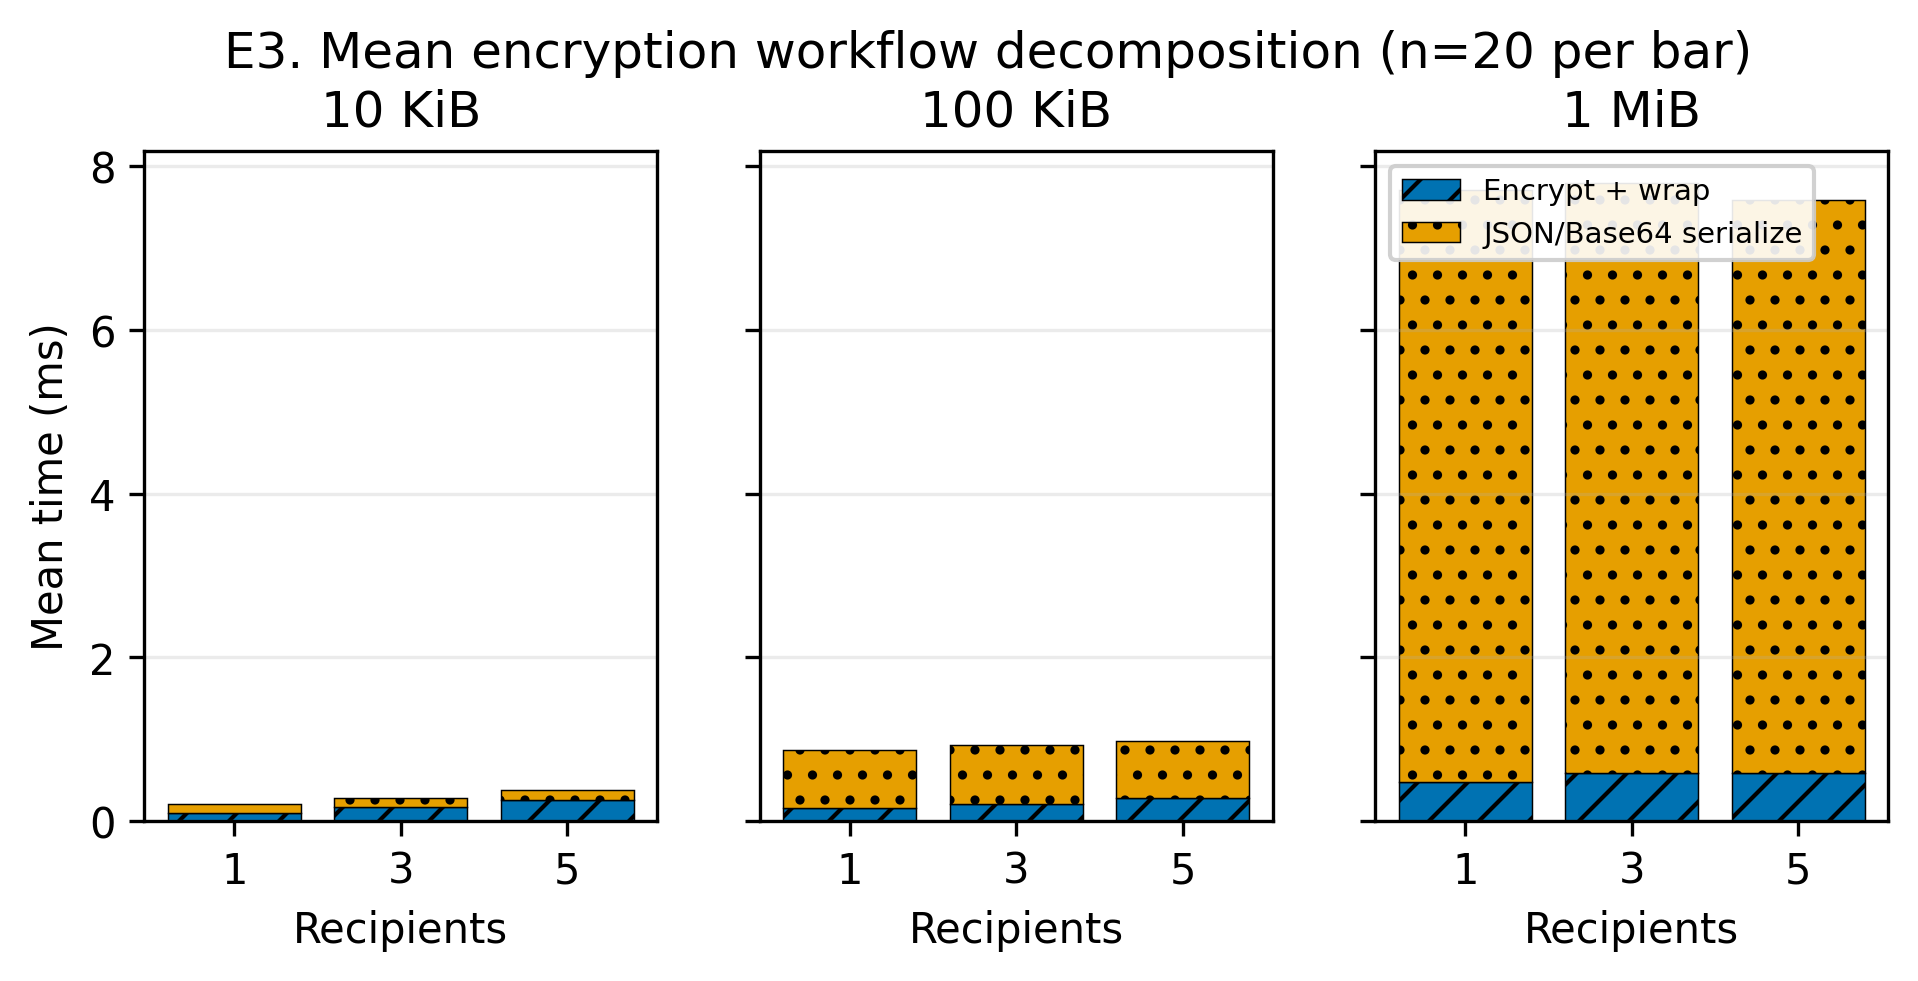
\includegraphics[width=\linewidth]{../docs/analysis/figures/figure_3_e3_timing_decomposition.png}
\caption{Mean E3 encrypt+wrap and JSON/Base64 serialization durations in milliseconds, 20 timed repetitions per file-size/recipient configuration using prepared RSA keys. Panels have independently labeled, zero-based Y scales. Routine total encryption is the sum of these two components; recipient-key generation was timed separately.}
\label{fig:e3}
\end{figure}

Table~\ref{tab:e3} also reports medians and interquartile ranges (IQRs).

\begin{table}[!ht]
\centering\small
\caption{E3 total encryption workflow: descriptive timing statistics and serialized-package overhead. Each row has 20 timed repetitions; times are milliseconds. IQR is the recorded 75th minus 25th percentile. Key generation is excluded.}
\label{tab:e3}
\begin{tabular}{@{}llrrrr@{}}
\toprule
File & Recipients & Mean & Median & IQR & Overhead (\%) \\
\midrule
10\,KiB & 1 & 0.205 & 0.197 & 0.088 & 40.28 \\
        & 3 & 0.283 & 0.293 & 0.084 & 49.40 \\
        & 5 & 0.375 & 0.354 & 0.097 & 58.52 \\
100\,KiB & 1 & 0.870 & 0.848 & 0.135 & 34.03 \\
         & 3 & 0.934 & 0.867 & 0.132 & 34.94 \\
         & 5 & 0.985 & 0.960 & 0.106 & 35.85 \\
1\,MiB & 1 & 7.712 & 7.401 & 0.406 & 33.40 \\
        & 3 & 7.795 & 7.548 & 0.263 & 33.49 \\
        & 5 & 7.594 & 7.521 & 0.128 & 33.58 \\
\bottomrule
\end{tabular}
\end{table}
\FloatBarrier

The three 1\,MiB total means are 7.712, 7.795 and 7.594\,ms for one, three and five recipients. Their non-monotonic order does not establish a speed advantage for five recipients: the differences are small compared with measured variation and may reflect scheduling or interpreter effects. The decryption interval covers only the first valid recipient, not sequential decryption for all recipients.

The actual serialized package follows an accounting identity for the current canonical JSON format. If $L$ is plaintext length, $r$ is recipient count, $f$ is filename and $\mathcal I$ denotes recipient identifiers, then
\begin{equation}\label{eq:size}
P(L,r)=4\left\lceil\frac{L+16}{3}\right\rceil+H(L,r,f,\mathcal I).
\end{equation}
The first term is Base64 encoding of the $L$ encrypted content bytes plus the 16-byte GCM tag. $H$ covers JSON delimiters, algorithm/version labels, decimal file size, nonce, filename, fingerprints and a Base64-encoded 256-byte RSA-2048 wrapped AES key for each recipient. It is not constant for arbitrary filenames and identifiers. For the fixed E3 metadata the model matched every measured package size with zero residual because it reconstructs the serializer's exact structure; this is an accounting check, not an independently fitted law or a cryptographic proof. At 10\,KiB, observed overhead rises from 40.28\% with one recipient to 58.52\% with five. At 1\,MiB it is 33.40\% to 33.58\%: Base64's approximately one-third expansion dominates while per-recipient metadata becomes relatively smaller. AES-GCM's tag alone would add far less.
\FloatBarrier

\subsection{E4: selected failure and integrity cases}
All 11 correctness cases matched their expected status. The valid package with a matching recipient key returned the original bytes. Ten invalid, mismatched or modified inputs returned no plaintext: wrong private key, absent recipient ID, changed encrypted content, changed GCM tag, changed authenticated filename, changed nonce, changed wrapped key, shortened recipient list, unsupported version and malformed JSON. The observed API classified the last two as structural \texttt{invalid\_package} and the other eight as \texttt{decryption\_failed}. This classification does not claim to identify malicious intent or the exact cryptographic cause of every failure. The tests illustrate package validation and fail-closed behavior for selected inputs; they are not an estimate of a universal attack-rejection probability.
